\chapter{Motivación}


\section{Introducción}
En las capas anteriores hemos visto como la estructura tecnológica le da soporte a la arquitectura empresarial, pero en esta capa vamos a visualizar y a modelar las razones o motivaciones que subyacen al diseño de esta, ya que son estas motivaciones las que restringen y van guiando el diseño de esta.\\
Las motivaciones reales están representadas por metas, principios, requisitos y restricciones.Las metas buscan representar algún resultado deseado - o fin - que una parte interesada desea lograr; por ejemplo, aumentar la satisfacción del cliente. 
Los principios y requisitos representan las propiedades deseadas de soluciones  o medios  mediante los cuales se pueden alcanzar los objetivos. 
Los principios son una serie de normativas  o pautas que guían el diseño de todas las soluciones posibles en un contexto dado. Y finalmente los requisitos representan declaraciones formales de necesidad, expresada por las partes interesadas, que debe cumplir la arquitectura o las soluciones siendo estas últimas inamovibles.\\
\\
\\
\\
\\
\\
\\
\\
\\
\\
\\
\\
\\
\\



\section{Punto de Vista de StakeHolder}
\subsection{Descripción}
El punto de vista de las partes interesadas permite identificar y modelas los impulsores internos y externos para el cambio y las evaluaciones (en términos de fortalezas, debilidades, oportunidades y (amenazas) de estos controladores. 
Además, los enlaces al objetivo inicial (alto nivel)  que abordan estos preocupaciones y evaluaciones pueden ser descritas. Estos objetivos forman la base del proceso de ingeniería de requerimientos, que incluye el refinamiento de objetivos, el análisis de contribución y conflicto, y la derivación de requisitos que cumplan los objetivos.


\subsubsection{Metamodelo}
\begin{figure}[h]
	\centering
	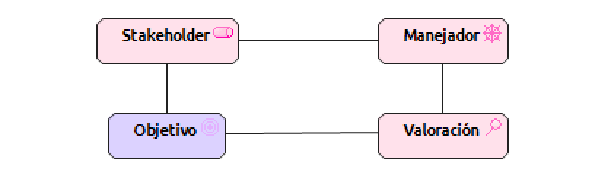
\includegraphics[width=1.0\textwidth]{imagenes/Metamodelos/Motivacion/meta_Stakeholder.pdf}
	\caption{Metamodelo: Punto de Vista de StakeHolder}
	\label{fig:gap_analysis}
\end{figure}

\subsubsection{Caso de Estudio}
El diagrama de Stakeholder o “partes interesadas” aplicado al caso de estudio, genera el modelo que se presenta a continuación, en el visualizamos nuestro objetivo de alto nivel correspondiente a “Mantener el vehículo Seguro” este objetivo presenta las partes interesadas representadas en el cliente y el representante de la empresa que en este caso es el guardia de turno, todo esto buscando que se fortalezca la percepción de seguridad en el cliente.

\begin{figure}[h]
	\centering
	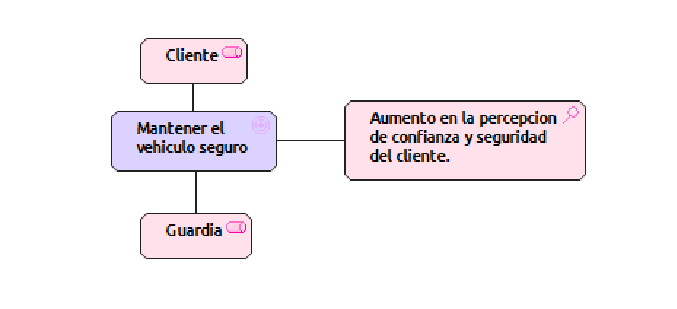
\includegraphics[width=1.0\textwidth]{imagenes/Caso_Estudio/Motivacion/Stakeholder.PDF}
	\caption{Caso de estudio: Punto de Vista de StakeHolder.}
	\label{fig:gap_analysis}
\end{figure}



\section{Punto de Vista de Realización de Objetivos}
\subsection{Descripción}
El punto de vista de realización de objetivos permite a un diseñador modelar el refinamiento de objetivos (de alto nivel) en objetivos más tangibles, y el refinamiento de objetivos tangibles en requisitos o restricciones que describen las propiedades que se necesitan para alcanzar los objetivos. El refinamiento de las metas en sub objetivos se modela utilizando la relación de agregación. El refinamiento de las metas en requisitos se modela utilizando la relación de realización. 
\subsubsection{Metamodelo}
\begin{figure}[h]
	\centering
	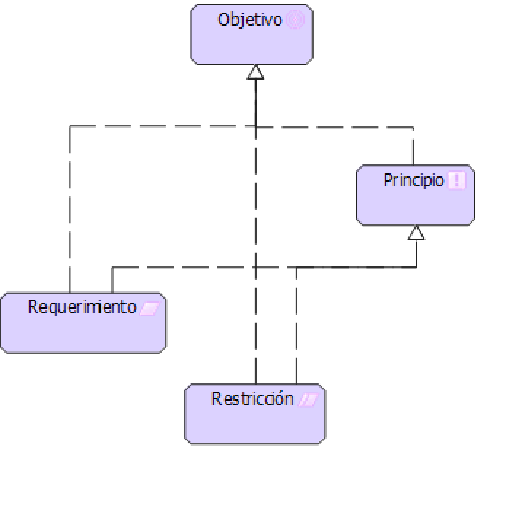
\includegraphics[width=0.7\textwidth]{imagenes/Metamodelos/Motivacion/meta_realizacion_objetivos.pdf}
	\caption{Metamodelo: Punto de Vista de Realización de Objetivos}
	\label{fig:gap_analysis}
\end{figure}

\subsubsection{Caso de Estudio}
Para el modelamiento del diagrama de realización de objetivos tenemos al igual que en el diagrama de Stakeholder el objetivo de alto nivel “Mantener seguro el vehículo”, adicional a esto encontramos una serie de restricciones que se deben cumplir para que el objetivo sea ejecutado exitosamente, ejemplo de ello es el requerimiento: “El vehículo solo se puede retirar si se ha efectuado el pago del servicio” esta restricción nos lleva a plantear el requerimiento de que la transacción del pago sea exitosa.

\begin{figure}[h]
	\centering
	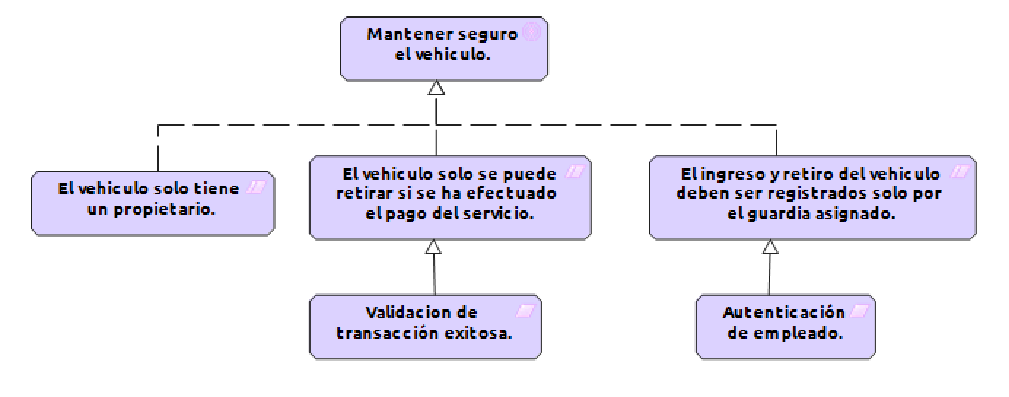
\includegraphics[width=1.0\textwidth]{imagenes/Caso_Estudio/Motivacion/Realizacion_Objetivos.PDF}
	\caption{Caso de estudio: Punto de Vista de Realización de Objetivos.}
	\label{fig:gap_analysis}
\end{figure}

\section{Punto de Vista de Contribución}
\subsection{Descripción}
El punto de vista de contribución permite modelar las relaciones de influencia entre objetivos y los requisitos necesarios para llevarlos a buen puerto. Este punto de vista se puede usar para analizar el impacto que los objetivos tienen entre sí o para detectar conflictos entre los objetivos de los Stakeholders. Este punto de vista requiere un refinamiento de los objetivos en lo posible un desglose lo mas detallado posible en sub objetivos. Al igual que en el punto de vista anterior tenemos los bloque y las relaciones de agregación y realización.

\subsubsection{Metamodelo}
\begin{figure}[h]
	\centering
	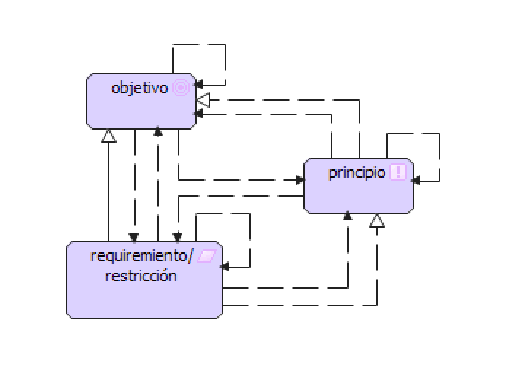
\includegraphics[width=0.8\textwidth]{imagenes/Metamodelos/Motivacion/meta_Contribucion.pdf}
	\caption{Metamodelo: Punto de Vista de Contribución.}
	\label{fig:gap_analysis}
\end{figure}

\subsubsection{Caso de Estudio}
Para el caso de uso y la implementación de este punto de vista, tenemos el objetivo principal el cual es mantener el vehículo seguro; adicional a esto se tiene el requerimiento de que se mantenga el estado estético y funcional de ingreso del vehículo, para esto vemos la influencia de objetivos secundarios o de bajo nivel lo cuales a su vez son restringidos e influenciados, tanto de manera positiva como de manera negativa.
\\
\\
\\
\\
\\
\\
\\
\\
\\
\\
\\

\begin{figure}[h]
	\centering
	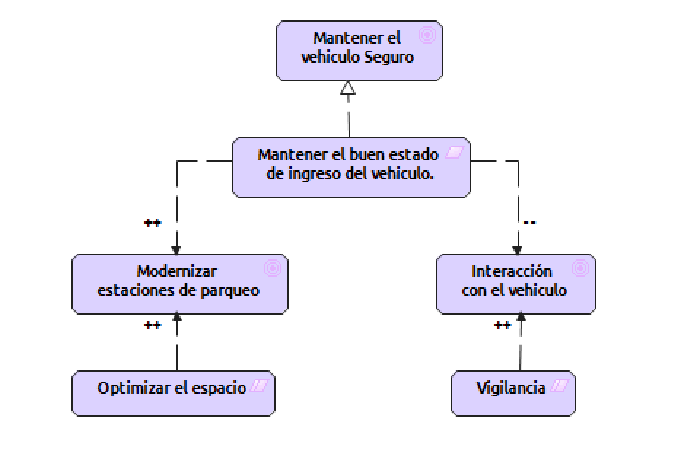
\includegraphics[width=0.8\textwidth]{imagenes/Caso_Estudio/Motivacion/Contribucion.PDF}
	\caption{Caso de estudio: Punto de Vista de Contribución.}
	\label{fig:gap_analysis}
\end{figure}

\section{Punto de Vista de Principios}
\subsection{Descripción}
El punto de vista de los principios permite modelar los principios más  influyentes o relevantes que dan  solución al problema de diseño en cuestión, también incluye los objetivos que motivan dicho modelamiento, adicionalmente los principios pueden influenciarse mutua y bilateralmente tanto de manera positiva como de manera negativa.
\subsubsection{Metamodelo}
\begin{figure}[h]
	\centering
	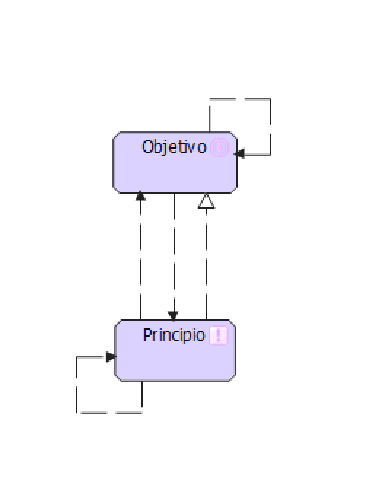
\includegraphics[width=0.4\textwidth]{imagenes/Metamodelos/Motivacion/meta_Principios.pdf}
	\caption{Metamodelo: Punto de Vista de Principios.}
	\label{fig:gap_analysis}
\end{figure}

\begin{figure}[h]
	\centering
	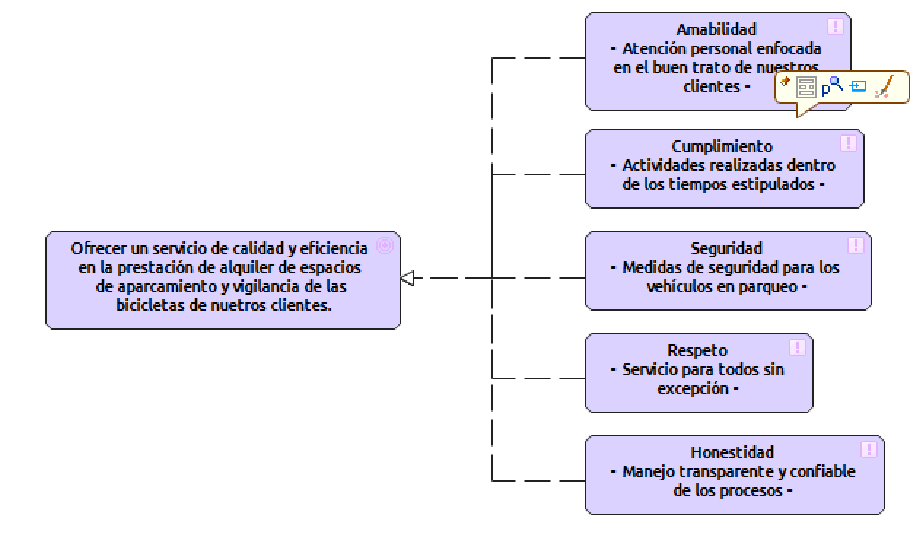
\includegraphics[width=0.8\textwidth]{imagenes/Caso_Estudio/Motivacion/Principios.PDF}
	\caption{Caso de estudio: Punto de Vista de Principios.}
	\label{fig:gap_analysis}
\end{figure}

\subsubsection{Caso de Estudio}
En este punto de vista se presentan los principios que serán piezas clave para el completo cumplimiento del objetivo principal de la empresa Two Wheels Parking. Podemos resaltar entre ellos el principio de Seguridad, el cual forma parte importante de la misión de la organización, y el principio de Cumplimiento que obliga las actividades sean realizadas dentro de los tiempos establecidos, favoreciendo la eficiencia en los procesos de la compañía.

\section{Punto de Vista de Realización de Requerimientos}
\subsection{Descripción}
El punto de vista de realización de requisitos nos permite centrarnos un poco más en el modelamiento y la realización de los requisitos que afectan a los elementos centrales, como son los actores comerciales, los servicios comerciales, las empresas, procesos, servicios de aplicaciones, componentes de aplicaciones, etc… Al igual que los puntos de vista anteriores en este también se evidencia la facilidad con la cual se puede abstraer más información logrando así un refinamiento en este caso de los requisitos.

\subsubsection{Metamodelo}
\begin{figure}[h]
	\centering
	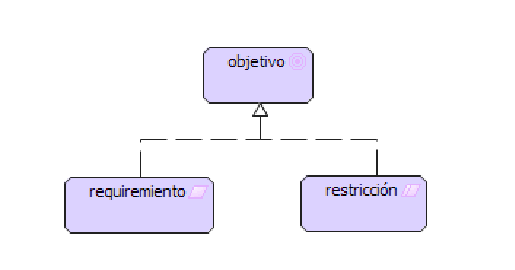
\includegraphics[width=0.6\textwidth]{imagenes/Metamodelos/Motivacion/meta_Realizacion_Requerimientos.pdf}
	\caption{Metamodelo: Punto de Vista de Realización de Requerimientos.}
	\label{fig:gap_analysis}
\end{figure}

\subsubsection{Caso de Estudio}
Con el fin de llevar a cabo el principal objetivo de la organización, se deben cumplir requerimientos y restricciones asociados a este. De estos podemos resaltar el requerimiento relacionado con la dotación y el personal necesarios para realizar un correcto control de la vigilancia y seguridad de los vehículos parqueados. Así también el requerimiento y la restricción asociados a la gestión de los espacios de parqueo.

\begin{figure}[h]
	\centering
	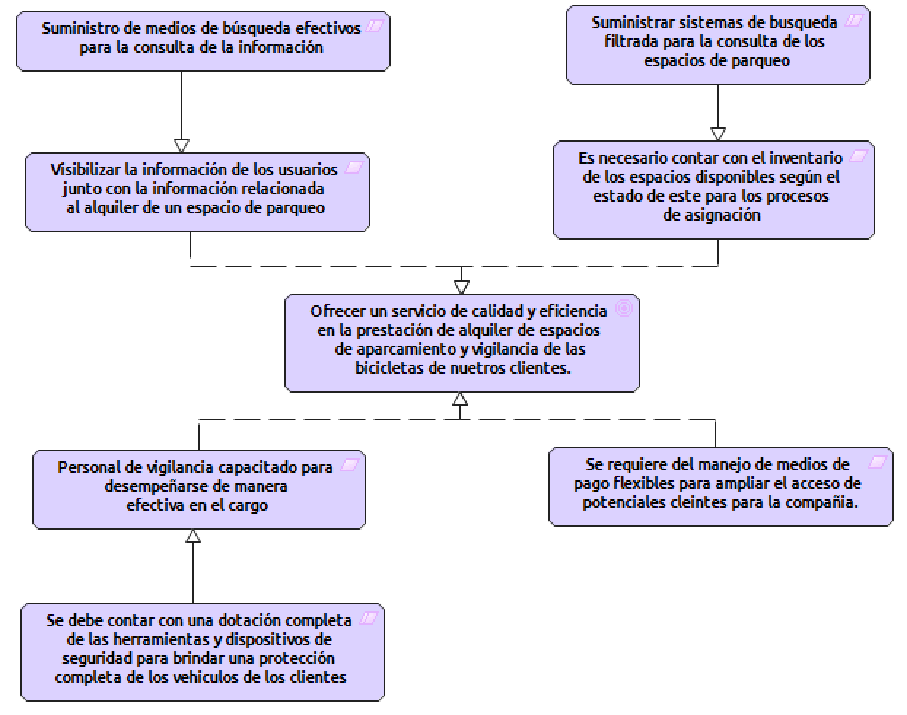
\includegraphics[width=1.0\textwidth]{imagenes/Caso_Estudio/Motivacion/Realizacion_Requerimientos.PDF}
	\caption{Caso de estudio: Punto de Vista de Realización de Requerimientos.}
	\label{fig:gap_analysis}
\end{figure}


\section{Punto de Vista de Motivación}
\subsection{Descripción}
El punto de vista de motivación es una mirada general de manera completa o parcial, esto teniendo en cuenta que hay ciertos elementos dentro de su aspecto que pasan a un segundo plano, es importante recalcar que a demás de esto también hacen presencia los interesados o Stakeolders junto a sus objetivos principales.
\\
\\
\\
\\
\\
\\
\\
\subsubsection{Metamodelo}
\begin{figure}[h]
	\centering
	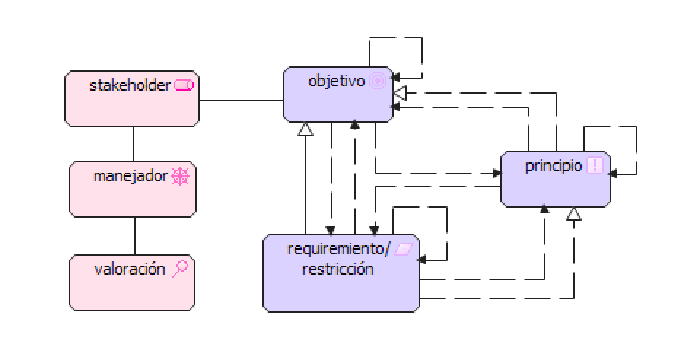
\includegraphics[width=1.0\textwidth]{imagenes/Metamodelos/Motivacion/meta_Motivacion.pdf}
	\caption{Metamodelo: Punto de Vista de Motivación.}
	\label{fig:gap_analysis}
\end{figure}

\subsubsection{Caso de Estudio}
En el siguiente punto de vista se destacan dos roles primordiales de la organización: El cajero, quien cumple el objetivo de asesorar en el proceso de alquiler de los espacios de parqueo sujeto a la realización de una serie de requerimientos asociados a los procesos de atención al cliente. Por otro lado, el Personal de Seguridad, quien desempeña funciones que garantizan la protección de los vehículos parqueados y cumple un objetivo específico relacionado con la vigilancia y seguridad de dichos vehículos.

\begin{figure}[h]
	\centering
	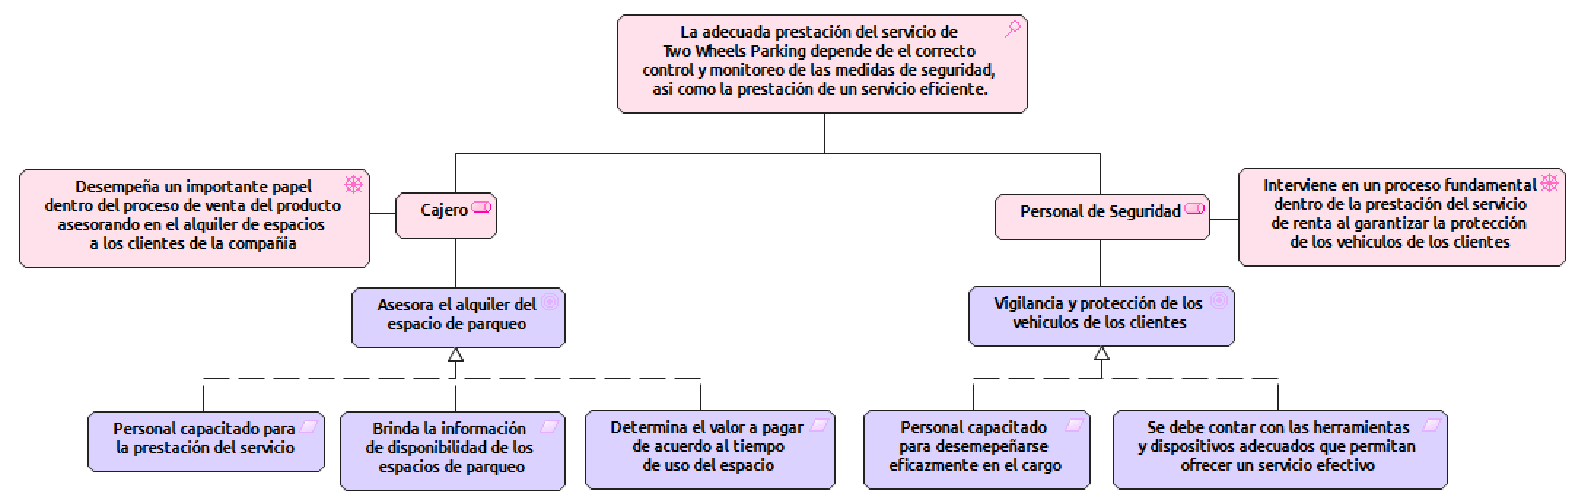
\includegraphics[width=1.0\textwidth]{imagenes/Caso_Estudio/Motivacion/Motivacion.PDF}
	\caption{Caso de estudio: Punto de Vista de Motivación.}
	\label{fig:gap_analysis}
\end{figure}


